\section{Photonik Sensoren}
\subsection{Helligkeits-Sensoren}
\subsubsection{Fotowiderstände LDR (Light Dependent Resistor)}
Trifft Licht auf die fotoempfindliche Fläche des Fotowiderstands, verringert sich der Widerstand durch den inneren fotoelektrischen Effekt. D.h. ein eintreffendes Photon hebt ein Elektron in das Leitungsband, welches sich nun frei im Kristall bewegen kann: Das Material wird niederohmiger. LDR's haben den Nachteil, dass sie ziemlich wärmeempfindlich und träge sind (Der Dunkelwiderstand wird erst nach $\frac{1}{60}s$ wieder erreicht).

\subsubsection{Photodiode}
\begin{wrapfigure}[14]{l}{0.5\textwidth}
    \vspace{-12pt}
    \centering
    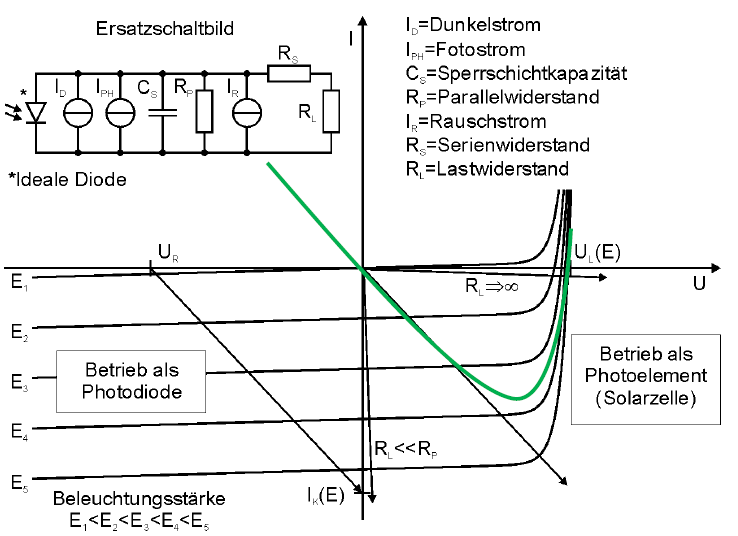
\includegraphics[width=0.48\textwidth]{images/photodiode}
\end{wrapfigure}
Treffen Photonen mit ausreichender Energie auf einen pn-Übergang, so werden Ladungsträger (Elektron-Loch-Paare) erzeugt. In der Raumladungszone driften die Ladungsträger schnell entgegen der Diffusionsspannung in die gleichartig dotierten Zonen, und führen zu einem Strom. Ohne externe Verbindung der Anschlüsse entsteht an diesen eine messbare Spannung gleicher Polarität wie die Durchflussspannung (Sättigung). Sind die Anschlüsse miteinander elektrisch verbunden oder befinden sie sich an einer Spannung in Sperrrichtung der Diode, fliesst ein Photostrom, der proportional zum Lichteinfall ist. Die Photonen müssen eine höhere Energie als die des Bandabstandes aufweisen, um diesen Effekt hervorzurufen.

\subsection{Solarzellen}
Eine Photodiode kann als Solarzelle betrieben werden. Dabei gibt es die folgenden Betriebsmodi:
\begin{compactitem}
    \item ohne Last: Sättigung mit Leerlaufspannung $U_L$, $U_L$ hängt dabei wenig von der Lichtstärke ab
    \item mit niederohmiger Last: Bei kleinerem $R_L$ sinkt Spannung und Strom steigt (bis max. Kurzschlussstrom $I_K$)
    \item bei MPP: Am Knick der Kennlinie liegt der angestrebte Arbeitspunkt MPP (Maximum Power Point) mit max. Leistung. Der MPP liegt dabei bei ca. 80\% Leerlaufspannung.
\end{compactitem}

\subsection{Photodiode als Lichtsensor}
\subsubsection{Betrieb im Quasi-Kurzschluss (U = 0)}
\begin{wrapfigure}[5]{l}{0.25\textwidth}
    \vspace{-12pt}
    \centering
    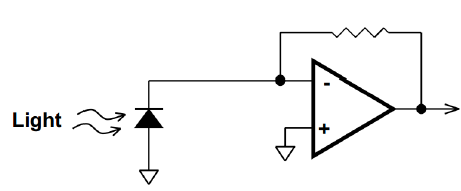
\includegraphics[width=0.22\textwidth]{images/photodiode_betrieb_01}
\end{wrapfigure}
Der Photo-Strom wird in Sperrrichtung erzeugt und ist linear abhängig von der Bestrahlungsstärke. Der Opamp ist als Transimpedanzverstärker geschaltet. Es erfolgt keine Änderung der Spannung und keine Umladung von Kapazitäten. Dadurch ist die Schaltung relativ schnell. Die grosse Diodenkapazität ist aber ein Problem für den Opamp. 

\subsubsection{Betrieb im Sperrbereich}
\begin{wrapfigure}[4]{l}{0.25\textwidth}
    \vspace{-12pt}
    \centering
    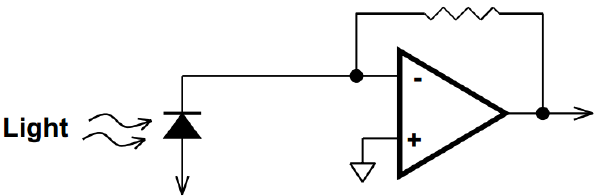
\includegraphics[width=0.22\textwidth]{images/photodiode_betrieb_02}
\end{wrapfigure}
Es liegt eine negative Spannung über der Photodiode. Die Diodenkapazität ist dadurch kleiner und die Schaltung schneller. Der Dunkelstrom $I_D$ steigt hingegen mit Spannung und Temperatur an. Er überlagert den Photostrom und bestimmt das Rauschen.

\subsection{Phototransistor}
Phototransistoren sind wesentlich empfindlicher als Photodioden, die Basis-Emitter-Diode ist eine Photodiode. Der Photostrom wird verstärkt mit dem Stromverstärkungsfaktor $\beta$. Allerdings sind sie viel langsamer als Photodioden.

\subsection{Spektrale Empfindlichkeit}
Silizium ist am empfindlichsten bei ca. 850nm, wird aber für gesamtes Spektrum von blau bis NIR (400nm – 900nm) genutzt. Andere Wellenlängen bedingen aufwändigere Herstellungsprozesse mit zusätzlichen Dotierungen.

\subsubsection{Eindringtiefe der Photonen}
Je nach Wellenlänge dringt das Licht mehr oder weniger tief ins Halbleitermaterial ein. Bei Silizium ergeben sich z.B. folgende Eindringtiefen:
\begin{compactitem}
    \item blau, $400nm$: $a = 2*10^4cm^{-1}$ $\rightarrow$ $d=500nm$
    \item rot, $700nm$: $a = 5*10^3cm^{-1}$ $\rightarrow$ $d=2um$
    \item infrarot, $1000nm$: $a = 3*10^2cm^{-1}$ $\rightarrow$ $d=33um$
\end{compactitem}

\subsubsection{CMOS-IC-Prozesse mit Fotodioden}
\begin{multicols}{4}
    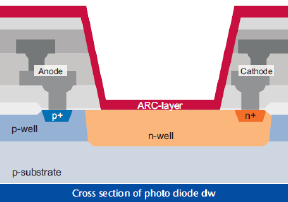
\includegraphics[width=0.24\textwidth]{images/eindringtiefe_01}
    Standard Diode in jedem Prozess vorhanden, maximum bei Rot \\
    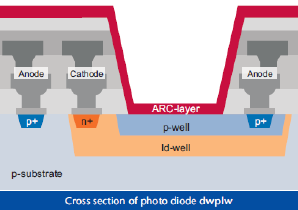
\includegraphics[width=0.24\textwidth]{images/eindringtiefe_02}
    Zweite Diode näher an der Si-Oberfläche, bessere Blau-Empfindlichkeit \\
    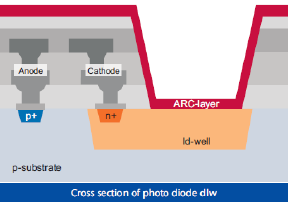
\includegraphics[width=0.24\textwidth]{images/eindringtiefe_03}
    Low-doped NWell: Depletionszone tiefer im Substrat, mehr IR-Empfindlichkeit \\
    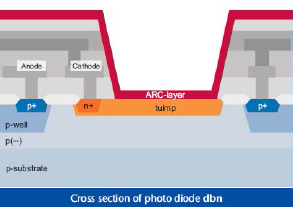
\includegraphics[width=0.24\textwidth]{images/eindringtiefe_04}
    Sehr dünne, oberflächennahe Implantierung, Blau-und UV-Empfindlich (DVD, Blueray-Empfänger)
\end{multicols}

Für kürzere Wellenlängen (UV+Röntgen) wird ein Scintillator-Kristall(z.B. CäsiumIodidCsI) auf die Diode aufgebracht: Die Strahlung regt den Kristall an, welcher dann bei einer längeren Wellenlänge im sichtbaren Bereich leuchtet.

\subsection{Avalanche-Photodioden}
\begin{wrapfigure}[11]{l}{0.35\textwidth}
    \vspace{-12pt}
    \centering
    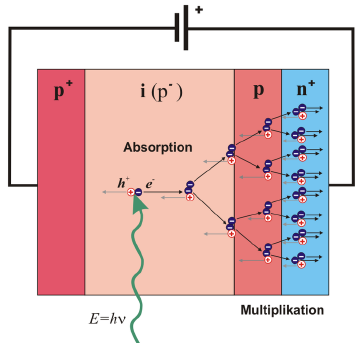
\includegraphics[width=0.34\textwidth]{images/apd}
\end{wrapfigure}
Avalanche-Photodioden sind hochempfindlich und schnell. Sie nutzen den inneren photoelektrischen Effekt zur Ladungsträgererzeugung und den Lawinendurchbruch (Avalanche-Effekt) zur internen Verstärkung. Eine Detektierung von sehr geringer Strahlung ist möglich (bis hin zu einzelnen Photonen). Die spektrale Empfindlichkeit liegt je nach verwendetem Material in einem Bereich von ca. 250 – 1700nm.
\subsubsection{Aufbau}
Photonen werden in der vollständig verarmten intrinsischen i-Schicht absorbiert und erzeugen dort Ladungsträgerpaare. In einer Si-APD werden die Elektronen zur Multiplikationszone hin beschleunigt und verursachen dort die Ladungslawine.

\subsection{CCD (Charge-Coupled-Device)}
\subsubsection{Funktionsweise}
\begin{multicols}{3}
    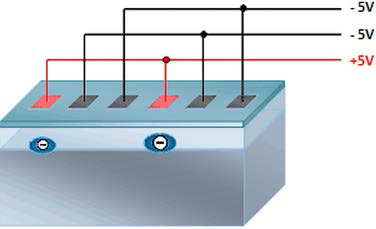
\includegraphics[width=0.32\textwidth]{images/ccd_01}
    Elektronen werden angezogen unter (rote) Elektroden mit pos. Spannung \\
    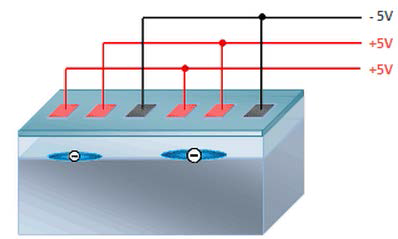
\includegraphics[width=0.32\textwidth]{images/ccd_02}
    Benachbarte Elektroden aktiviert: Elektronen verteilen sich unter 2 Elektroden \\
    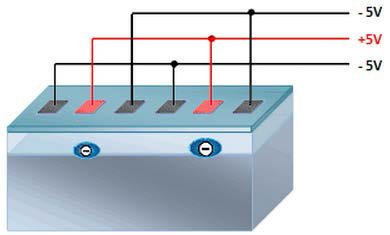
\includegraphics[width=0.32\textwidth]{images/ccd_03}
    Linke Elektrode deaktiviert, Elektronen sammeln sich unter nächster Elektrode \\
\end{multicols}
\begin{multicols}{3}
    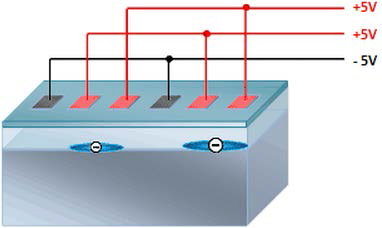
\includegraphics[width=0.32\textwidth]{images/ccd_04}
    Benachbarte Elektroden aktiviert, Elektronen verteilen sich wieder unter 2 Elektroden \\
    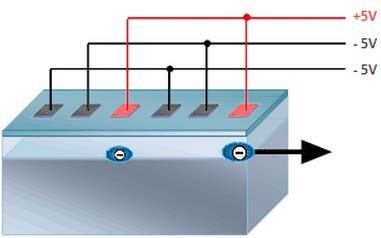
\includegraphics[width=0.32\textwidth]{images/ccd_05}
    Elektronen sind am Rand des Schieberegisters, Weiterverarbeitung mit Ladungsverstärker, ADC \\
    Die Frequenz, wie oft der Sensor pro Sekunde der in der Lage ist, die Ladung um einen Pixel weiter zu transportieren, wird "Pixel clock" genannt. Die Frequenzen, mit den CCDs heute betrieben werden, betragen rund 25 bis 50 MHz. \\ \ \\ \ \\ \ \\
\end{multicols}

\subsubsection{Auslesevarianten}
\begin{multicols}{2}
    \paragraph{Interline Transfer Sensor}
    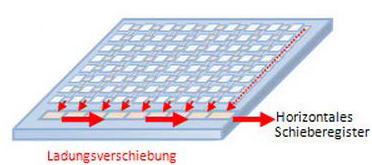
\includegraphics[width=0.39\textwidth]{images/ccd_interline} \\
    Bei dieser Variante erfolgt eine Trennung von Pixel und Speicherzellen. Der fillfactor des Sensors beträgt nur etwa 30 Prozent. Mikrolinsen helfen aber die Lichtausbeute zu erhöhen.
    
    \paragraph{Fullframe Transfer Sensor}
    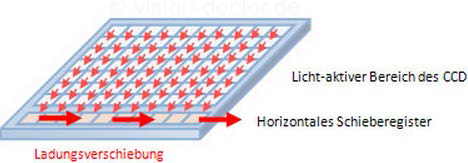
\includegraphics[width=0.49\textwidth]{images/ccd_fullframe}
    Die komplette Sensorfläche ist lichtaktiv. Er ist ideal für eine maximale Helligkeitsempfindlichkeit und er besitzt keine vertikalen Schieberegister. 
\end{multicols}

\subsubsection{Farb-Filter}
\begin{wrapfigure}[7]{l}{0.25\textwidth}
    \vspace{-12pt}
    \centering
    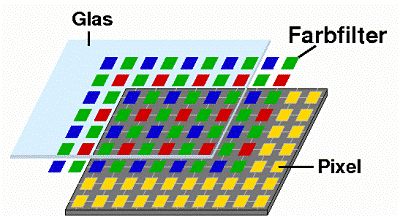
\includegraphics[width=0.24\textwidth]{images/ccd_filter}
\end{wrapfigure}
Die meisten Sensoren werden mit einem optischen Filter betrieben. Ein oft eingesetzter Filter basiert auf dem Bayer-Pattern. Dieses enthält 50\% grüne, 25\% blaue und 25\% rote Farbfilter. Ein De-Mosaicing ist anschliessend noch nötig. \\
In einer Alternativlösung wird anstelle eines Filters die unterschiedliche Eindringtiefe von Licht mit unterschiedlicher Wellenlänge ausgenutzt. Dabei besteht ein Pixel aus 3 gestackten Fotodioden. Dabei geht kein Licht verloren, die Separation ist aber schlecht.

\subsection{CMOS-Bildsensoren}
\subsubsection{Active Pixel Sensor (APS)}
\begin{wrapfigure}[15]{l}{0.25\textwidth}
    \vspace{-12pt}
    \centering
    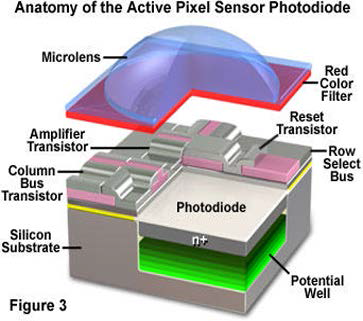
\includegraphics[width=0.24\textwidth]{images/cmos_aps}
    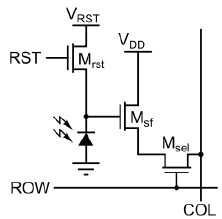
\includegraphics[width=0.24\textwidth]{images/cmos_aps_aufbau}
\end{wrapfigure}
Die Umwandlung von Ladung in Spannung geschieht innerhalb des Pixels. Jedes Pixel hat deshalb seine eigene Auslese-Elektronik. Dadurch ist ein flexibles auslesen (Region-of-Interest (ROI)) möglich. 
\paragraph{Funktionsweise}
Eine Zelle besteht aus einer Photodiode und 3 NMOS-Transistoren. Die Photodiode wird im Reset auf eine hohe Spannung gesetzt. Der Photostrom entlädt die Diodenkapazität, dies führt zu einer Integration des Photostromes während der Integrationszeit. Der Source-Follower-Transistor ($M_{sf}$) folgt der Diodenspannung (verschoben um konstante Spannung $V_{TH}$). Nach der Integrationszeit wird die Spannung am Pixel über den Source-Follower gemessen und über $M_{sel}$ ausgelesen. Jeweils eine ganze Zeile wird mit dem Reset-Transistor zurückgesetzt. Mit dem Selekt-Transistor wird eine einzelne Zeile aus dem Bildfeld angewählt. Jede Ausgangskolonne hat einen eigenen Kolonnen-Verstärker. Teilweise wandeln Kolonnen-ADC's das Signal direkt in ein digitales Signal um. Ein Kolonnenmultiplexer selektiert am Schluss eine Kolonne nach der anderen und gibt das Signal an den Ausgang aus. \\

\paragraph{Rauschen im Pixel}
\begin{wrapfigure}[15]{r}{0.45\textwidth}
    \vspace{-12pt}
    \centering
    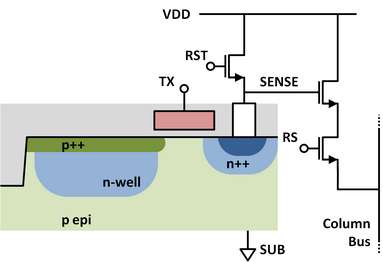
\includegraphics[width=0.43\textwidth]{images/cmos_aps_pinned}
\end{wrapfigure}
Wird ein Knoten über einen Transistor auf ein Potential gesetzt und der Transistor danach geöffnet, so ist das Potential auf dem Knoten rauschbehaftet. Die Rauschspannung kann dabei folgendermassen berechnet werden: $V_{n, kTC} = \sqrt{\frac{kT}{C}}$. Die Anzahl der Rauschelektronen kann ebenfalls bestimmt werden: $n_{n, kTC} = \frac{\sqrt{kT*C}}{q}$ \\
Dies kann verhindert werden indem durch einen zusätzlichen Layer $p++$ die Photodiode gepinnt wird. Dabei ist die Photodiode vom Ausleseknoten über das Gate TX getrennt. Wird TX auf high gesetzt, fliesst alle Ladung in den Ausleseknoten. Dies erlaubt Correlated Double Sampling (CDS) und eliminiert das Reset-oder $\frac{kT}{C}$-Rauschen.

\paragraph{Global Shutter Pixel}
Bei einem Rolling Shutter Pixel werden sich schnell bewegende Objekte falsch aufgenommen. Aus diesem Grund gibt es Global Shutter Pixel. Diese haben einen zusätzlichen Sense-Node (SN). Bei dieser Art werden alle Pixel gleichzeitig zurückgesetzt und die integrierte Ladung aller Pixel werden gleichzeitig auf den Sense-Node übertragen. Dabei integrieren alle Pixel über den exakt selben Zeitraum, die Bewegungen werden eingefroren. Ein Nachteil ist, dass die Photodiode kleiner wird bei gleichbleibender Pixelfläche.

\begin{wrapfigure}[15]{l}{0.5\textwidth}
    \vspace{-12pt}
    \centering
    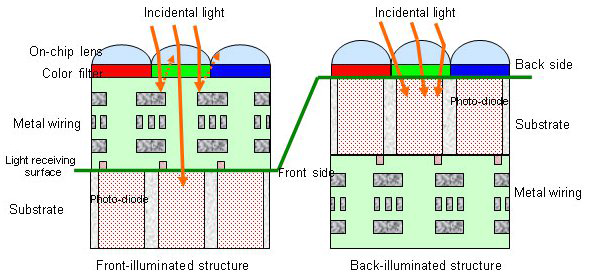
\includegraphics[width=0.48\textwidth]{images/cmos_iluminated}
\end{wrapfigure}
\paragraph{Front- und Back-illuminated CMOS}
\begin{compactitem}
    \item Front-illuminated Sensoren: Metall-Verbindungen absorbieren Licht 
    \item Back-illuminated Sensoren: Höhere Lichtausbeute
\end{compactitem}

